

\title{\LARGE \bf
Dimentionless Policies based on the Buckingham $\pi$ Theorem: \\ 
Is it a good way to Generalize Numerical Results?
}


%\author{Alexandre~Girard,~\IEEEmembership{Member,~IEEE,}
%        and~H.~Harry~Asada,~\IEEEmembership{Member,~IEEE}% <-this % stops a space
\author{Alexandre Girard$^{1}$% <-this % stops a space
\thanks{$^{1}$Alexandre Girard is with the Department of Mechanical Engineering, Universite de Sherbrooke, Qc, Canada {\tt\small  alex.girard@usherbrooke.ca }}% <-this % stops a space
}%


% make the title area
\maketitle
\thispagestyle{empty}
\pagestyle{empty}


\begin{abstract}
Maybe. Here we show that by modifying the problem formulation of the pendulum swing-up task using dimentionless variables, we can re-use the optimal policy generated numerically for any pendulum that are dimentionnaly similar. We also demonstrate that by leveraging this scheme when using reinforcement learning, multiple systems of various dimentions can share a data-base during the learning phase, which can be a big advantage for data efficiency. It remains to be seen if this approach can also help generalizing policies for more complex high-dimentional problems.
\end{abstract}

%%%%%%%%%%%%%%%%%%%%%%
\section{Introduction}

Many numerical algorithms = black box mapping

System and problem parameters are not explicitly in the function




%%%%%%%%%%%%%%%%%%%%%%%%%%%%%%%%%%%%%%%%%%%%
\subsection{What define a policy?}

- steady states \\
- fully observable


For a specific system, a control policy 
%%%%%%%%%%%%%%%%%%%%%%
\begin{equation}
u
=
\pi \left(
x
\right)
\end{equation}
%%%%%%%%%%%%%%%%%%%%%%


%%%%%%%%%%%%%%%%%%%%%%
\begin{equation}
u
=
\pi \left(
x,
\theta_s,
\theta_p
\right)
\end{equation}
%%%%%%%%%%%%%%%%%%%%%%




%%%%%%%%%%%%%%%%%%%%%%
\begin{equation}
\pi \left(
x,
\theta_s,
\theta_p
\right)
\quad \Rightarrow \quad
\pi \left(
x,
\theta_s',
\theta_p'
\right)
\end{equation}
%%%%%%%%%%%%%%%%%%%%%%

%%%%%%%%%%%%%%%%%%%%%%
\begin{figure}[H]
\begin{center}
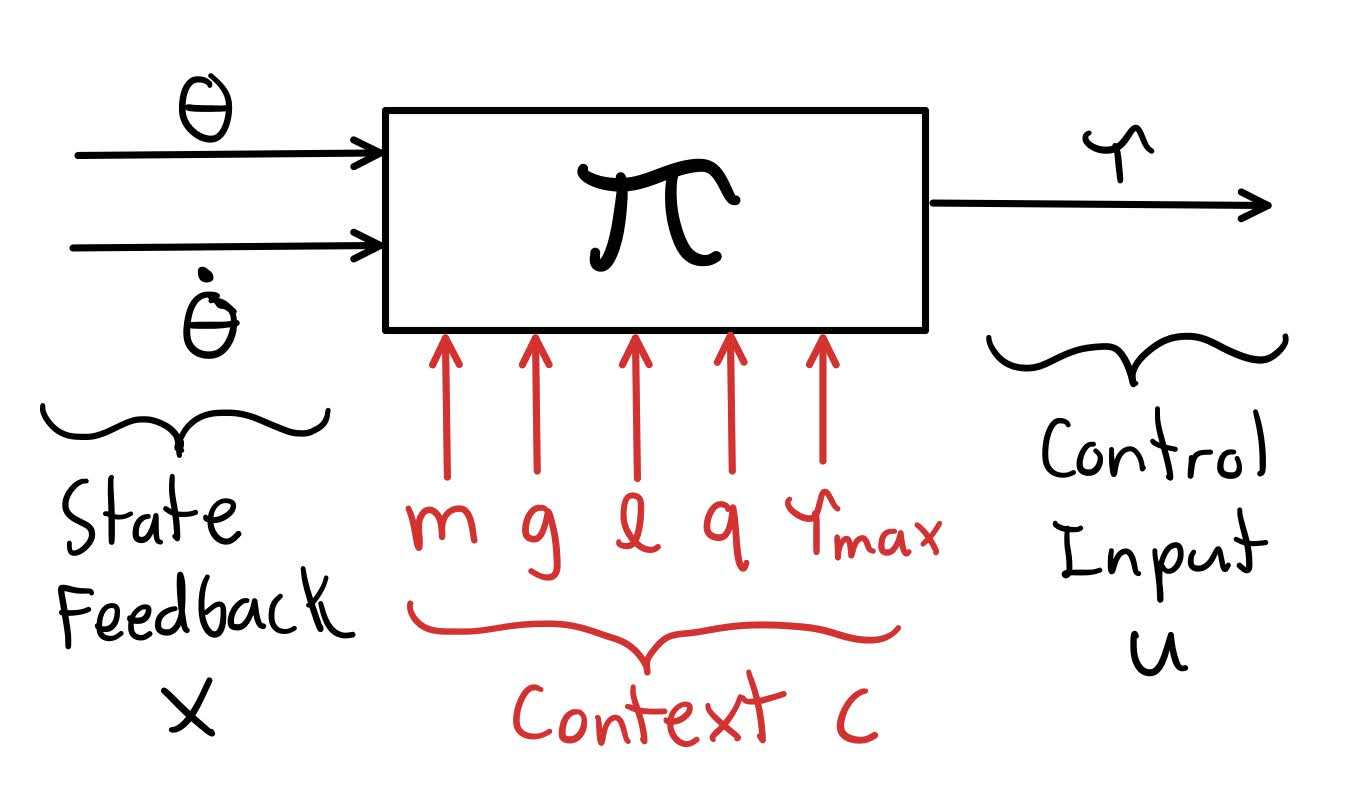
\includegraphics[width=0.99\linewidth]{fig/policy_context2.jpg}
\caption{Big picture}\label{fig:policy_context}
\end{center}
\end{figure}
%%%%%%%%%%%%%%%%%%%%%%

% %%%%%%%%%%%%%%%%%%%%%%
% \begin{figure}[H]
% \begin{center}
% 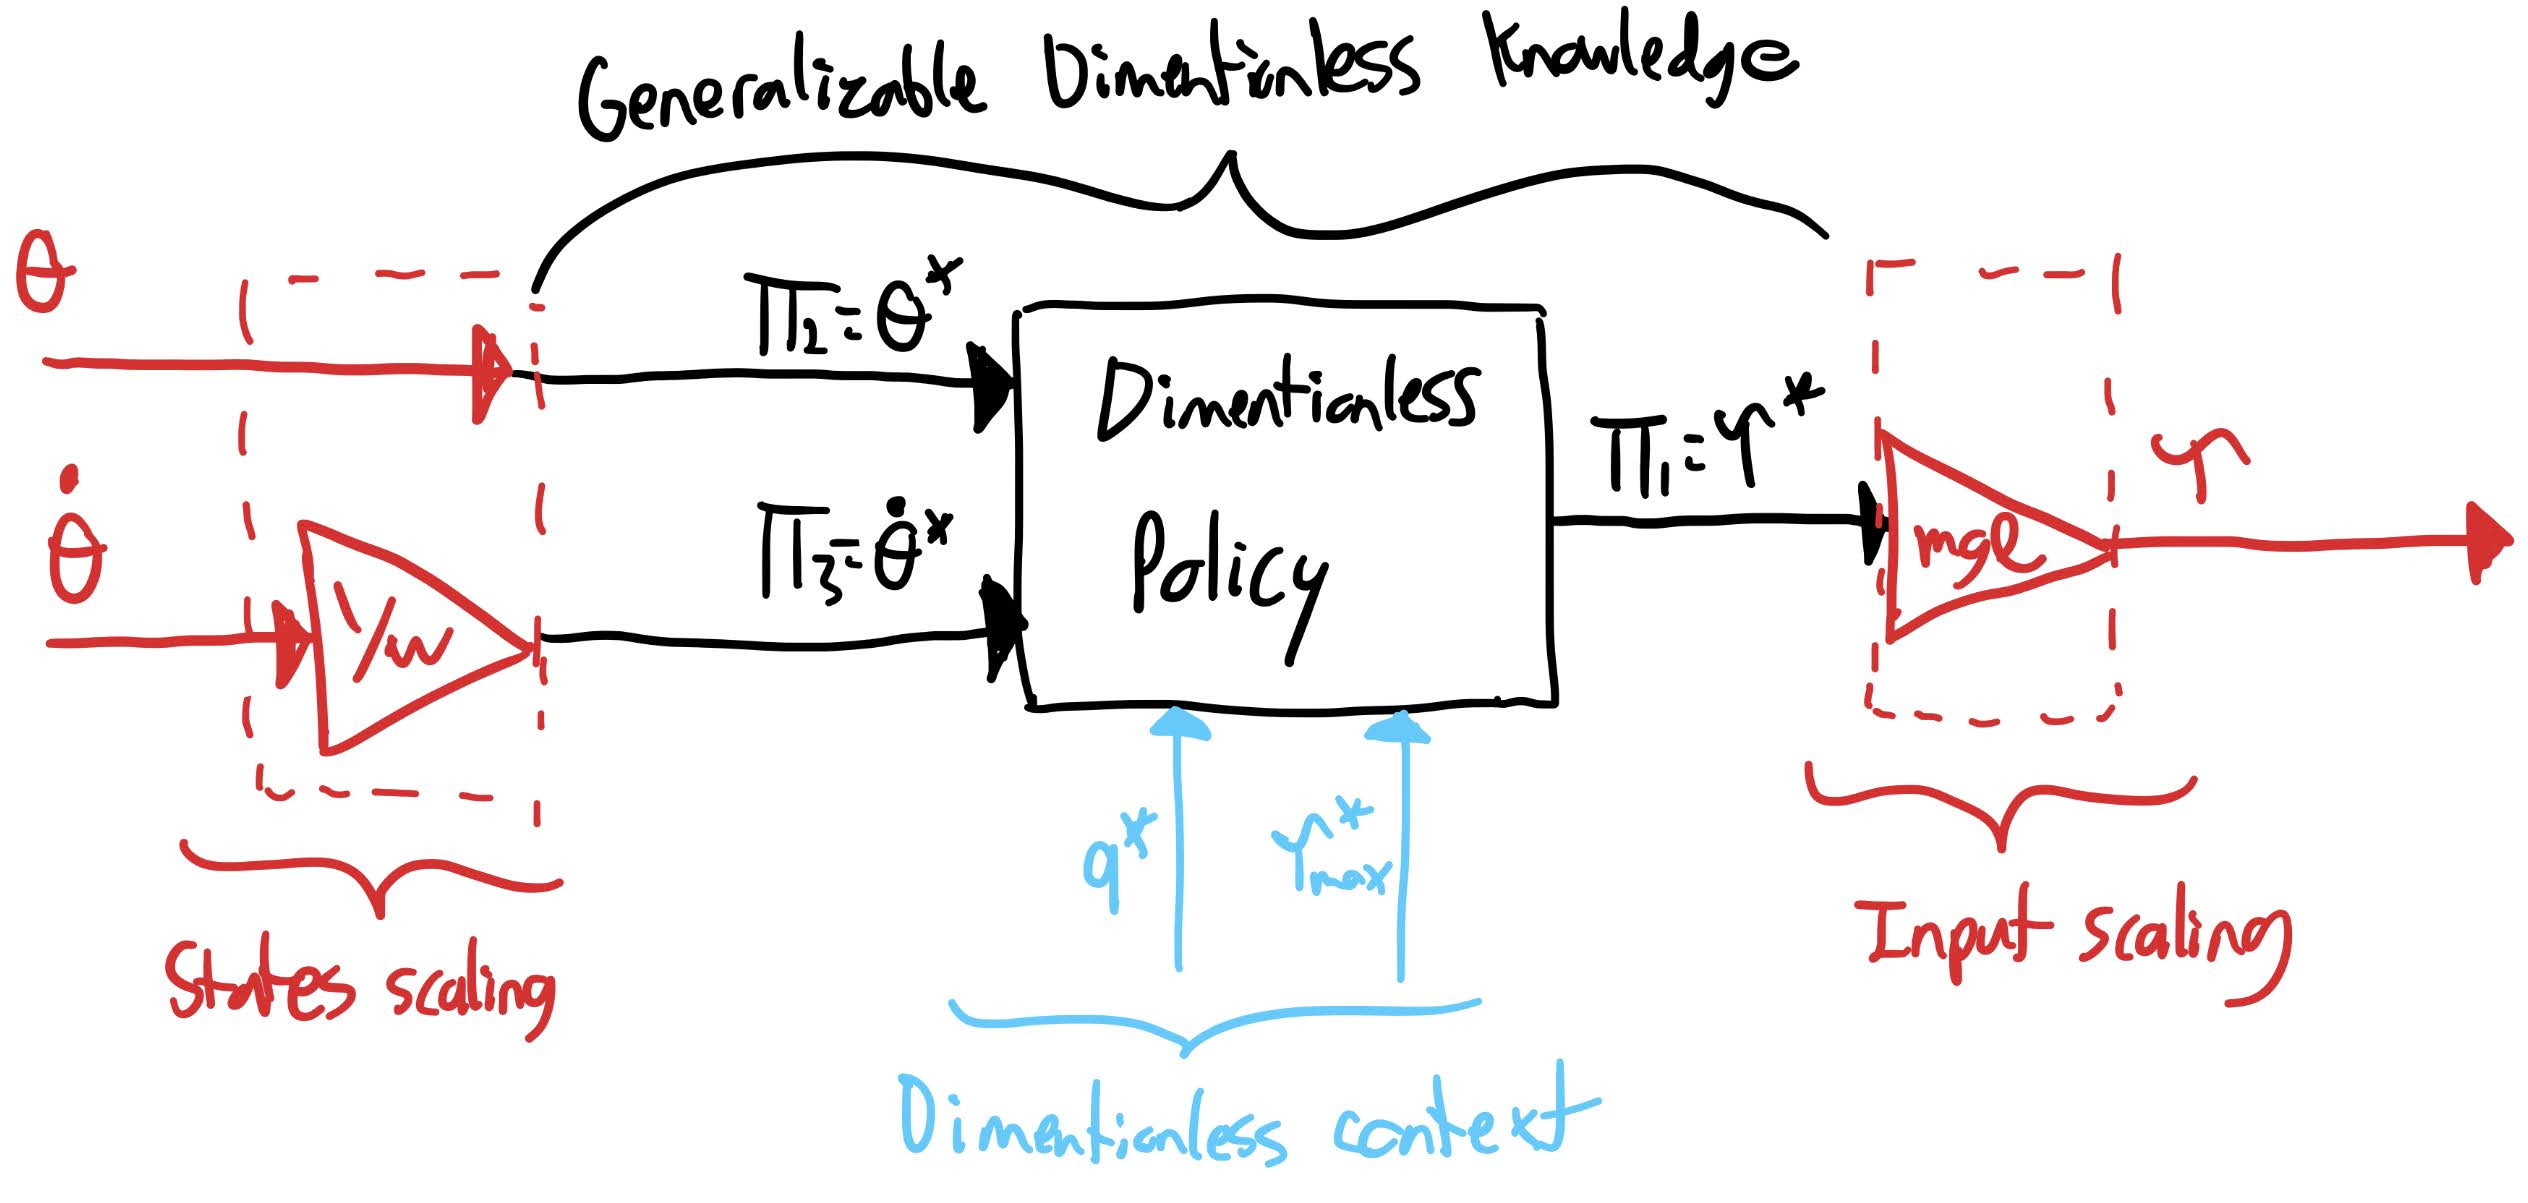
\includegraphics[width=0.99\linewidth]{fig/dim_policy_context.jpg}
% \caption{Goal = isolating the commun knowledge to facilitate reusing it}\label{fig:dim_policy_context}
% \end{center}
% \end{figure}
% %%%%%%%%%%%%%%%%%%%%%%

\subsection{Direct vs. indirect policy parameters}

Direct = policy parametrization

Indirect = policy is the results of an optimation, and the parameter are parametrizing a cost function with define the objective.


% %%%%%%%%%%%%%%%%%%%%%%
% \begin{equation}
% \underbrace{u}_{\text{inputs}}
% =
% \pi \left(
% \underbrace{x}_{\text{states}},
% \underbrace{\theta_s}_{\text{system parameters}},
% \underbrace{\theta_p}_{\text{policy parameters}}
% \right)
% \end{equation}
% %%%%%%%%%%%%%%%%%%%%%%

\newpage
%%%%%%%%%%%%%%%%%%%%%%
\section{Pendulum swing-up task}
In this paper, we will focus on solving a specific case study of the pendulum swing-up task. 

%%%%%%%%%%%%%%%%%%%%%%
\begin{equation}
\underbrace{\tau}_{\text{inputs}}
=
\pi \left(
\underbrace{ \theta, \dot{\theta} }_{\text{states}},
\underbrace{ m , g , l }_{\text{system parameters}},
\underbrace{ q , \tau_{max} }_{\text{policy parameters}}
\right)
\end{equation}
%%%%%%%%%%%%%%%%%%%%%%

The dynamic of the system is described by:
%%%%%%%%%%%%%%%%%%%%%%
\begin{equation}
ml^2 \ddot{\theta} + mgl \sin \theta = \tau
\end{equation}
%%%%%%%%%%%%%%%%%%%%%%

The cost function to minimize is given by:
%%%%%%%%%%%%%%%%%%%%%%
\begin{equation}
J = \int{( q^2 \theta^2 + 0 \, \dot{\theta}^2 + 1 \, \tau^2 ) dt }
\end{equation}
%%%%%%%%%%%%%%%%%%%%%%

Constraints on control inputs are given by:
%%%%%%%%%%%%%%%%%%%%%%
\begin{equation}
- \tau_{max} \leq \tau \leq \tau_{max}
\end{equation}
%%%%%%%%%%%%%%%%%%%%%%

\begin{table}[htb]
   \centering % center the table
   \caption{Pendulum swing-up optimal policy variables} 
   \label{expVari}
   \begin{tabular}{p{0.8cm} p{2.5cm} p{0.8cm} p{1.5cm} }
   \hline \hline \noalign{\smallskip} \noalign{\smallskip} \noalign{\smallskip} \noalign{\smallskip}
   %%%%%%%%%%%%%%%%%%%%%%
   \textbf{Variable} & \textbf{Description} & \textbf{Units} & \textbf{Dimensions} \\ 
   %%%%%%%%%%%%%%%%%%%%%%
   \hline \hline \noalign{\smallskip} 
   \multicolumn{4}{c}{\textbf{Control inputs}}\\ \noalign{\smallskip}  \hline \hline
   \noalign{\smallskip} 
   %%%%%%%%%%%%%%%%%%%%%%
   $\tau$ & Actuator torque & $Nm$ & [$ML^2T^{-2}$]\\ 
   %%%%%%%%%%%%%%%%%%%%%%
   \hline \hline \noalign{\smallskip} 
   \multicolumn{4}{c}{\textbf{State variables}}\\ \noalign{\smallskip}  \hline \hline \noalign{\smallskip} 
   %%%%%%%%%%%%%%%%%%%%%%
   $\theta$ & Joint angle & $rad$ & []\\ \noalign{\smallskip} \hline \noalign{\smallskip}
   $\dot{\theta}$ & Joint angular velocity & $rad/sec$ & [$T^{-1}$] \\
   %%%%%%%%%%%%%%%%%%%%%%
   \hline \hline \noalign{\smallskip} 
   \multicolumn{4}{c}{\textbf{System parameters}}\\ \noalign{\smallskip}  \hline\hline  \noalign{\smallskip} 
   %%%%%%%%%%%%%%%%%%%%%%
   $m$ & Pendulum mass & $kg$ & [$M$]  \\ \noalign{\smallskip} \hline \noalign{\smallskip}
   $g$ & Gravity       & $m/s^2$ & [$LT^{-2}$]  \\ \noalign{\smallskip} \hline \noalign{\smallskip}
   $l$ & Pendulum lenght & $m$ & [$L$]  \\ \noalign{\smallskip} \hline \noalign{\smallskip}
%%%%%%%%%%%%%%%%%%%%%%
   \hline \hline \noalign{\smallskip} 
   \multicolumn{4}{c}{\textbf{Problem parameters}}\\ \noalign{\smallskip}  \hline\hline  \noalign{\smallskip} 
   %%%%%%%%%%%%%%%%%%%%%%
   $q$ & Weight parameter  & $Nm$ & [$ML^2T^{-2}$]   \\ \noalign{\smallskip} \hline \noalign{\smallskip}
   $\tau_{max}$ & Maximum torque & $Nm$ & [$ML^2T^{-2}$] \\ \noalign{\smallskip} \hline \noalign{\smallskip}
   \hline \noalign{\smallskip}
   %\bottomrule[\heavyrulewidth] 
   \end{tabular}
\end{table}

But here the 3 system paramters $m$, $g$ and $l$ are only present in two groups in the dynamic equation. 

\begin{table}[htb]
   \centering % center the table
   \caption{Pendulum swing-up optimal policy variables} 
   \label{expVari}
   \begin{tabular}{p{1.5cm} p{2.2cm} p{0.8cm} p{1.5cm} }
   \hline \hline \noalign{\smallskip} \noalign{\smallskip} \noalign{\smallskip} \noalign{\smallskip}
   %%%%%%%%%%%%%%%%%%%%%%
   \textbf{Variable} & \textbf{Description} & \textbf{Units} & \textbf{Dimensions} \\ 
   %%%%%%%%%%%%%%%%%%%%%%
   \hline \hline \noalign{\smallskip} 
   \multicolumn{4}{c}{\textbf{Control inputs}}\\ \noalign{\smallskip}  \hline \hline
   \noalign{\smallskip} 
   %%%%%%%%%%%%%%%%%%%%%%
   $\tau$ & Actuator torque & $Nm$ & [$ML^2T^{-2}$]\\ 
   %%%%%%%%%%%%%%%%%%%%%%
   \hline \hline \noalign{\smallskip} 
   \multicolumn{4}{c}{\textbf{State variables}}\\ \noalign{\smallskip}  \hline \hline \noalign{\smallskip} 
   %%%%%%%%%%%%%%%%%%%%%%
   $\theta$ & Joint angle & $rad$ & []\\ \noalign{\smallskip} \hline \noalign{\smallskip}
   $\dot{\theta}$ & Joint angular velocity & $rad/sec$ & [$T^{-1}$] \\
   %%%%%%%%%%%%%%%%%%%%%%
   \hline \hline \noalign{\smallskip} 
   \multicolumn{4}{c}{\textbf{System parameters}}\\ \noalign{\smallskip}  \hline\hline  \noalign{\smallskip} 
   %%%%%%%%%%%%%%%%%%%%%%
   $mgl$ & Maximum gravitational torque  & $Nm$ & [$ML^2T^{-2}$]  \\ \noalign{\smallskip} \hline \noalign{\smallskip}
   $\omega = {(\frac{g}{l})}^{1/2}$ & Natural frequency & $sec^{-1}$ & [$T^{-1}$]  \\ \noalign{\smallskip} \hline \noalign{\smallskip}
%%%%%%%%%%%%%%%%%%%%%%
   \hline \hline \noalign{\smallskip} 
   \multicolumn{4}{c}{\textbf{Problem parameters}}\\ \noalign{\smallskip}  \hline\hline  \noalign{\smallskip} 
   %%%%%%%%%%%%%%%%%%%%%%
   $q$ & Weight parameter  & $Nm$ & [$ML^2T^{-2}$]   \\ \noalign{\smallskip} \hline \noalign{\smallskip}
   $\tau_{max}$ & Maximum torque & $Nm$ & [$ML^2T^{-2}$] \\ \noalign{\smallskip} \hline \noalign{\smallskip}
   \hline \noalign{\smallskip}
   %\bottomrule[\heavyrulewidth] 
   \end{tabular}
\end{table}



%%%%%%%%%%%%%%%%%%%%%%%%%%%%%%%%%%%%%%%%%%%%
\subsection{Dimentionless dynamics}


% %%%%%%%%%%%%%%%%%%%%%%
% \begin{align}
% \ddot{\theta} &= \frac{\tau}{ml^2} - \frac{mgl}{ml^2} \sin \theta \\
% \ddot{\theta} &= \omega^2 \left( \frac{\tau}{mgl} - \sin \theta \right)
% \end{align}
% %%%%%%%%%%%%%%%%%%%%%%
%%%%%%%%%%%%%%%%%%%%%%
\begin{align}
%ml^2 \ddot{\theta} + mgl \sin \theta &= \tau  \\
\frac{\ddot{\theta}}{\omega^2} + \sin \theta &= \frac{\tau}{mgl}
\end{align}
%%%%%%%%%%%%%%%%%%%%%%

%%%%%%%%%%%%%%%%%%%%%%
\begin{equation}
m = (n = 5 ) - ( p = 2 ) = 3
\end{equation}
%%%%%%%%%%%%%%%%%%%%%%

%%%%%%%%%%%%%%%%%%%%%%
\begin{align}
\Pi_1 &= \tau^* = \frac{\tau}{mgl} \quad \quad \frac{[ML^2T^{-2}]}{[M][LT^{-2}][L]} \\
\Pi_2 &= \theta^* = \theta \quad \quad [-]\\
\Pi_3 &= \ddot{\theta}^* = \frac{ \ddot{\theta}  }{ \omega^2 } \quad \quad \frac{[T^{-2}]}{[T^{-1}][T^{-1}]} 
\end{align}
%%%%%%%%%%%%%%%%%%%%%%

% %%%%%%%%%%%%%%%%%%%%%%
% \begin{equation}
% \ddot{\theta}^*
% =
% f\left(
% \theta^*, \tau^* 
% \right) = \tau^* - \sin \theta
% \end{equation}
% %%%%%%%%%%%%%%%%%%%%%%
%%%%%%%%%%%%%%%%%%%%%%
\begin{equation}
\tau^*
=
f\left(
\theta^*,\ddot{\theta}^*
\right) = \ddot{\theta}^* + \sin \theta^*
\end{equation}
%%%%%%%%%%%%%%%%%%%%%%

\newpage 
\subsection{Applying the buckingham $\pi$ theorem to the policy function}

Here $n=7$ variables are involved and only $p=2$ independants dimensions ( $ML^2T^{-2}$ and $T^{-1}$ )

%%%%%%%%%%%%%%%%%%%%%%
\begin{equation}
m = (n = 7 ) - ( p = 2 ) = 5
\end{equation}
%%%%%%%%%%%%%%%%%%%%%%
Using $mgl$ and $\omega$, the system parameters, as the repeating variables lead to the following dimentionless groups:
%%%%%%%%%%%%%%%%%%%%%%
\begin{align}
\Pi_1 &= \tau^* = \frac{\tau}{mgl} \quad \quad \frac{[ML^2T^{-2}]}{[M][LT^{-2}][L]} \\
\Pi_2 &= \theta^* = \theta \quad \quad [-]\\
\Pi_3 &= \dot{\theta}^* = \frac{ \dot{\theta}  }{ \omega } \quad \quad \frac{[T^{-1}]}{[T^{-1}]} \\
\Pi_4 &= \tau_{max}^* = \frac{\tau_{max}}{mgl} \quad \quad \frac{[ML^2T^{-2}]}{[M][LT^{-2}][L]} \\
\Pi_5 &= q^* = \frac{q}{mgl} \quad \quad \frac{[Ml^2T^{-2}]}{[M][LT^{-2}][L]} 
\end{align}
%%%%%%%%%%%%%%%%%%%%%%
Here, all 3 torque variables (the system inputs, the system maximum and cost function parameter) are scaled by the maximum gravitationnal torque, and the pendulum velocity variable is scaled by the pendulum natural frequency.

%that corespond to torque required to balance the gravity when the pendulum is

According to the theorem, any policy that is only based on the variable included in our analysis can be expressed as a relationship between the 5 dimentionless pi groups in the form:

%%%%%%%%%%%%%%%%%%%%%%
\begin{equation}
\tau^*
=
\pi^* \left(
\theta, \dot{\theta}^*,
q^* , \tau_{max}^* 
\right)
\end{equation}
%%%%%%%%%%%%%%%%%%%%%%

\subsubsection{Interpretation}

\subsubsection{Impact on possible generalization}

In this context, the results means that for dimentionnally similar swing-up problem (which means here equal ratios $q^*$ and $\tau_{max}^*$), the optimal policy in dimentionnal form should be equivalent. In other words, if we have an optimal policy $\pi_1$ found in a specific context $\{m_1,l_1,g_1,q_1,\tau_{max,1}\}$, then the dimentionless control law of a second context $\{m_1,l_1,g_1,q_1,\tau_{max,1}\}$, should be the same if $q^*_1 = q^*_2$ and $\tau_{max,1}^* = \tau_{max,2}^*$, what we call \textit{dimentionnally similar}. However, if $q^*_1 \neq q^*_2$ or $\tau_{max,2}^* \neq \tau_{max,2}^*$ then $\pi_1$ doesn't give us more information on $\pi_2$.





\newpage
%%%%%%%%%%%%%%%%%%%%%%
\section{Closed-form parametric policies}

To better understand the concept of a dimentionless policy, here we first apply the buckingham pi theorem on well-known closed form solution.

\subsection{Computed torque}

The computed torque control law provide is a model-based policy that force the system (assuming no torque limits here) on a 2nd order exponential convergence on the desired trajectory:
%%%%%%%%%%%%%%%%%%%%%%
\begin{equation}
0 = (\ddot{\theta}_d - \ddot{\theta})+ 2 \omega_d \zeta (\dot{\theta}_d - \dot{\theta}) + \omega_d^2 (\theta - \theta)
\end{equation}
%%%%%%%%%%%%%%%%%%%%%%
For the specific case of the pendulum-swing up, the desired trajectory is simply the up-right position ($\ddot{\theta}_d = \dot{\theta}_d = \theta_d = 0$), and the control law takes this form:
%%%%%%%%%%%%%%%%%%%%%%
\begin{equation}
\tau = mgl \sin \theta - 2 m l^2 \omega_d \zeta \dot{\theta} - m l^2 \omega_d^2 \theta
\label{eq:ct}
\end{equation}
%%%%%%%%%%%%%%%%%%%%%%

%%%%%%%%%%%%%%%%%%%%%%
where the only parameters are the system parameters and two variables caracterizing the convergence speed. Hence, the torque policy is a function of those variables:
%%%%%%%%%%%%%%%%%%%%%%
\begin{equation}
\underbrace{\tau}_{\text{inputs}}
=
\pi_{ct} \left(
\underbrace{ \theta, \dot{\theta} }_{\text{states}},
\underbrace{ m , g , l }_{\text{system parameters}},
\underbrace{ \omega_d , \zeta }_{\text{policy parameters}}
\right)
\end{equation}
%%%%%%%%%%%%%%%%%%%%%%
having the dimension presented at table XXX.

%%%%%%%%%%%%%%%%%%%%%%%%%%%%%%%%%%%%%%%%%%%%
\begin{table}[htb]
   \centering % center the table
   \caption{Computed torque variables} 
   \label{expVari}
   \begin{tabular}{p{1.5cm} p{2.2cm} p{0.8cm} p{1.5cm} }
   \hline \hline \noalign{\smallskip} \noalign{\smallskip} \noalign{\smallskip} \noalign{\smallskip}
   %%%%%%%%%%%%%%%%%%%%%%
   \textbf{Variable} & \textbf{Description} & \textbf{Units} & \textbf{Dimensions} \\ 
   %%%%%%%%%%%%%%%%%%%%%%
   \hline \hline \noalign{\smallskip} 
   \multicolumn{4}{c}{\textbf{Control inputs}}\\ \noalign{\smallskip}  \hline \hline
   \noalign{\smallskip} 
   %%%%%%%%%%%%%%%%%%%%%%
   $\tau$ & Actuator torque & $Nm$ & [$ML^2T^{-2}$]\\ 
   %%%%%%%%%%%%%%%%%%%%%%
   \hline \hline \noalign{\smallskip} 
   \multicolumn{4}{c}{\textbf{State variables}}\\ \noalign{\smallskip}  \hline \hline \noalign{\smallskip} 
   %%%%%%%%%%%%%%%%%%%%%%
   $\theta$ & Joint angle & $rad$ & []\\ \noalign{\smallskip} \hline \noalign{\smallskip}
   $\dot{\theta}$ & Joint angular velocity & $rad/sec$ & [$T^{-1}$] \\
   %%%%%%%%%%%%%%%%%%%%%%
   \hline \hline \noalign{\smallskip} 
   \multicolumn{4}{c}{\textbf{System parameters}}\\ \noalign{\smallskip}  \hline\hline  \noalign{\smallskip} 
   %%%%%%%%%%%%%%%%%%%%%%
   $mgl$ & Maximum gravitational torque  & $Nm$ & [$ML^2T^{-2}$]  \\ \noalign{\smallskip} \hline \noalign{\smallskip}
   $\omega = {(\frac{g}{l})}^{1/2}$ & Natural frequency & $sec^{-1}$ & [$T^{-1}$]  \\ \noalign{\smallskip} \hline \noalign{\smallskip}
%%%%%%%%%%%%%%%%%%%%%%
   \hline \hline \noalign{\smallskip} 
   \multicolumn{4}{c}{\textbf{Policy parameters}}\\ \noalign{\smallskip}  \hline\hline  \noalign{\smallskip} 
   %%%%%%%%%%%%%%%%%%%%%%
   $\omega_d$ & Desired closed-loop frequency & $sec^{-1}$ & [$T^{-1}$]  \\ \noalign{\smallskip} \hline \noalign{\smallskip}
   $\zeta$ &  Desired closed-loop damping & $-$ & [ ]  \\ \noalign{\smallskip} \hline \noalign{\smallskip}
   \end{tabular}
\end{table}
%%%%%%%%%%%%%%%%%%%%%%%%%%%%%%%%%%%%%%%%%%%%
Here $n=7$ variables are involved and only $p=2$ independants dimensions ( $ML^2T^{-2}$ and $T^{-1}$ )
%%%%%%%%%%%%%%%%%%%%%%
\begin{equation}
m = (n = 7 ) - ( p = 2 ) = 5
\end{equation}
%%%%%%%%%%%%%%%%%%%%%%
Using $mgl$ and $\omega$, the system parameters, as the repeating variables lead to the following dimentionless groups:
%%%%%%%%%%%%%%%%%%%%%%
\begin{align}
\Pi_1 &= \tau^* = \frac{\tau}{mgl} \quad \quad \frac{[ML^2T^{-2}]}{[M][LT^{-2}][L]} \\
\Pi_2 &= \theta^* = \theta \quad \quad [-]\\
\Pi_3 &= \dot{\theta}^* = \frac{ \dot{\theta}  }{ \omega } \quad \quad \frac{[T^{-1}]}{[T^{-1}]} \\
\Pi_4 &= \omega_d^* = \frac{\omega_d}{\omega} \quad \quad \frac{[T^{-1}]}{[T^{-1}]} \\
\Pi_5 &= \zeta^* = \zeta \quad \quad []
\end{align}
%%%%%%%%%%%%%%%%%%%%%%



%%%%%%%%%%%%%%%%%%%%%%
\begin{equation}
\tau^*
=
\pi^*_{ct} \left(
\theta, \dot{\theta}^*,
\omega_d^* , \zeta^* 
\right)
\end{equation}
%%%%%%%%%%%%%%%%%%%%%%

Here we can confirme directly, dividing eq \eqref{eq:ct} by $mgl$ leads to :
%%%%%%%%%%%%%%%%%%%%%%
\begin{equation}
\tau^*
=
\sin \theta
- 2 \omega_d^* \zeta \dot{\theta}^* 
- (\omega_d^*)^2 \theta
\end{equation}
%%%%%%%%%%%%%%%%%%%%%%

%%%%%%%%%%%%%%%%%%%%%%
\begin{figure}[H]
\begin{center}
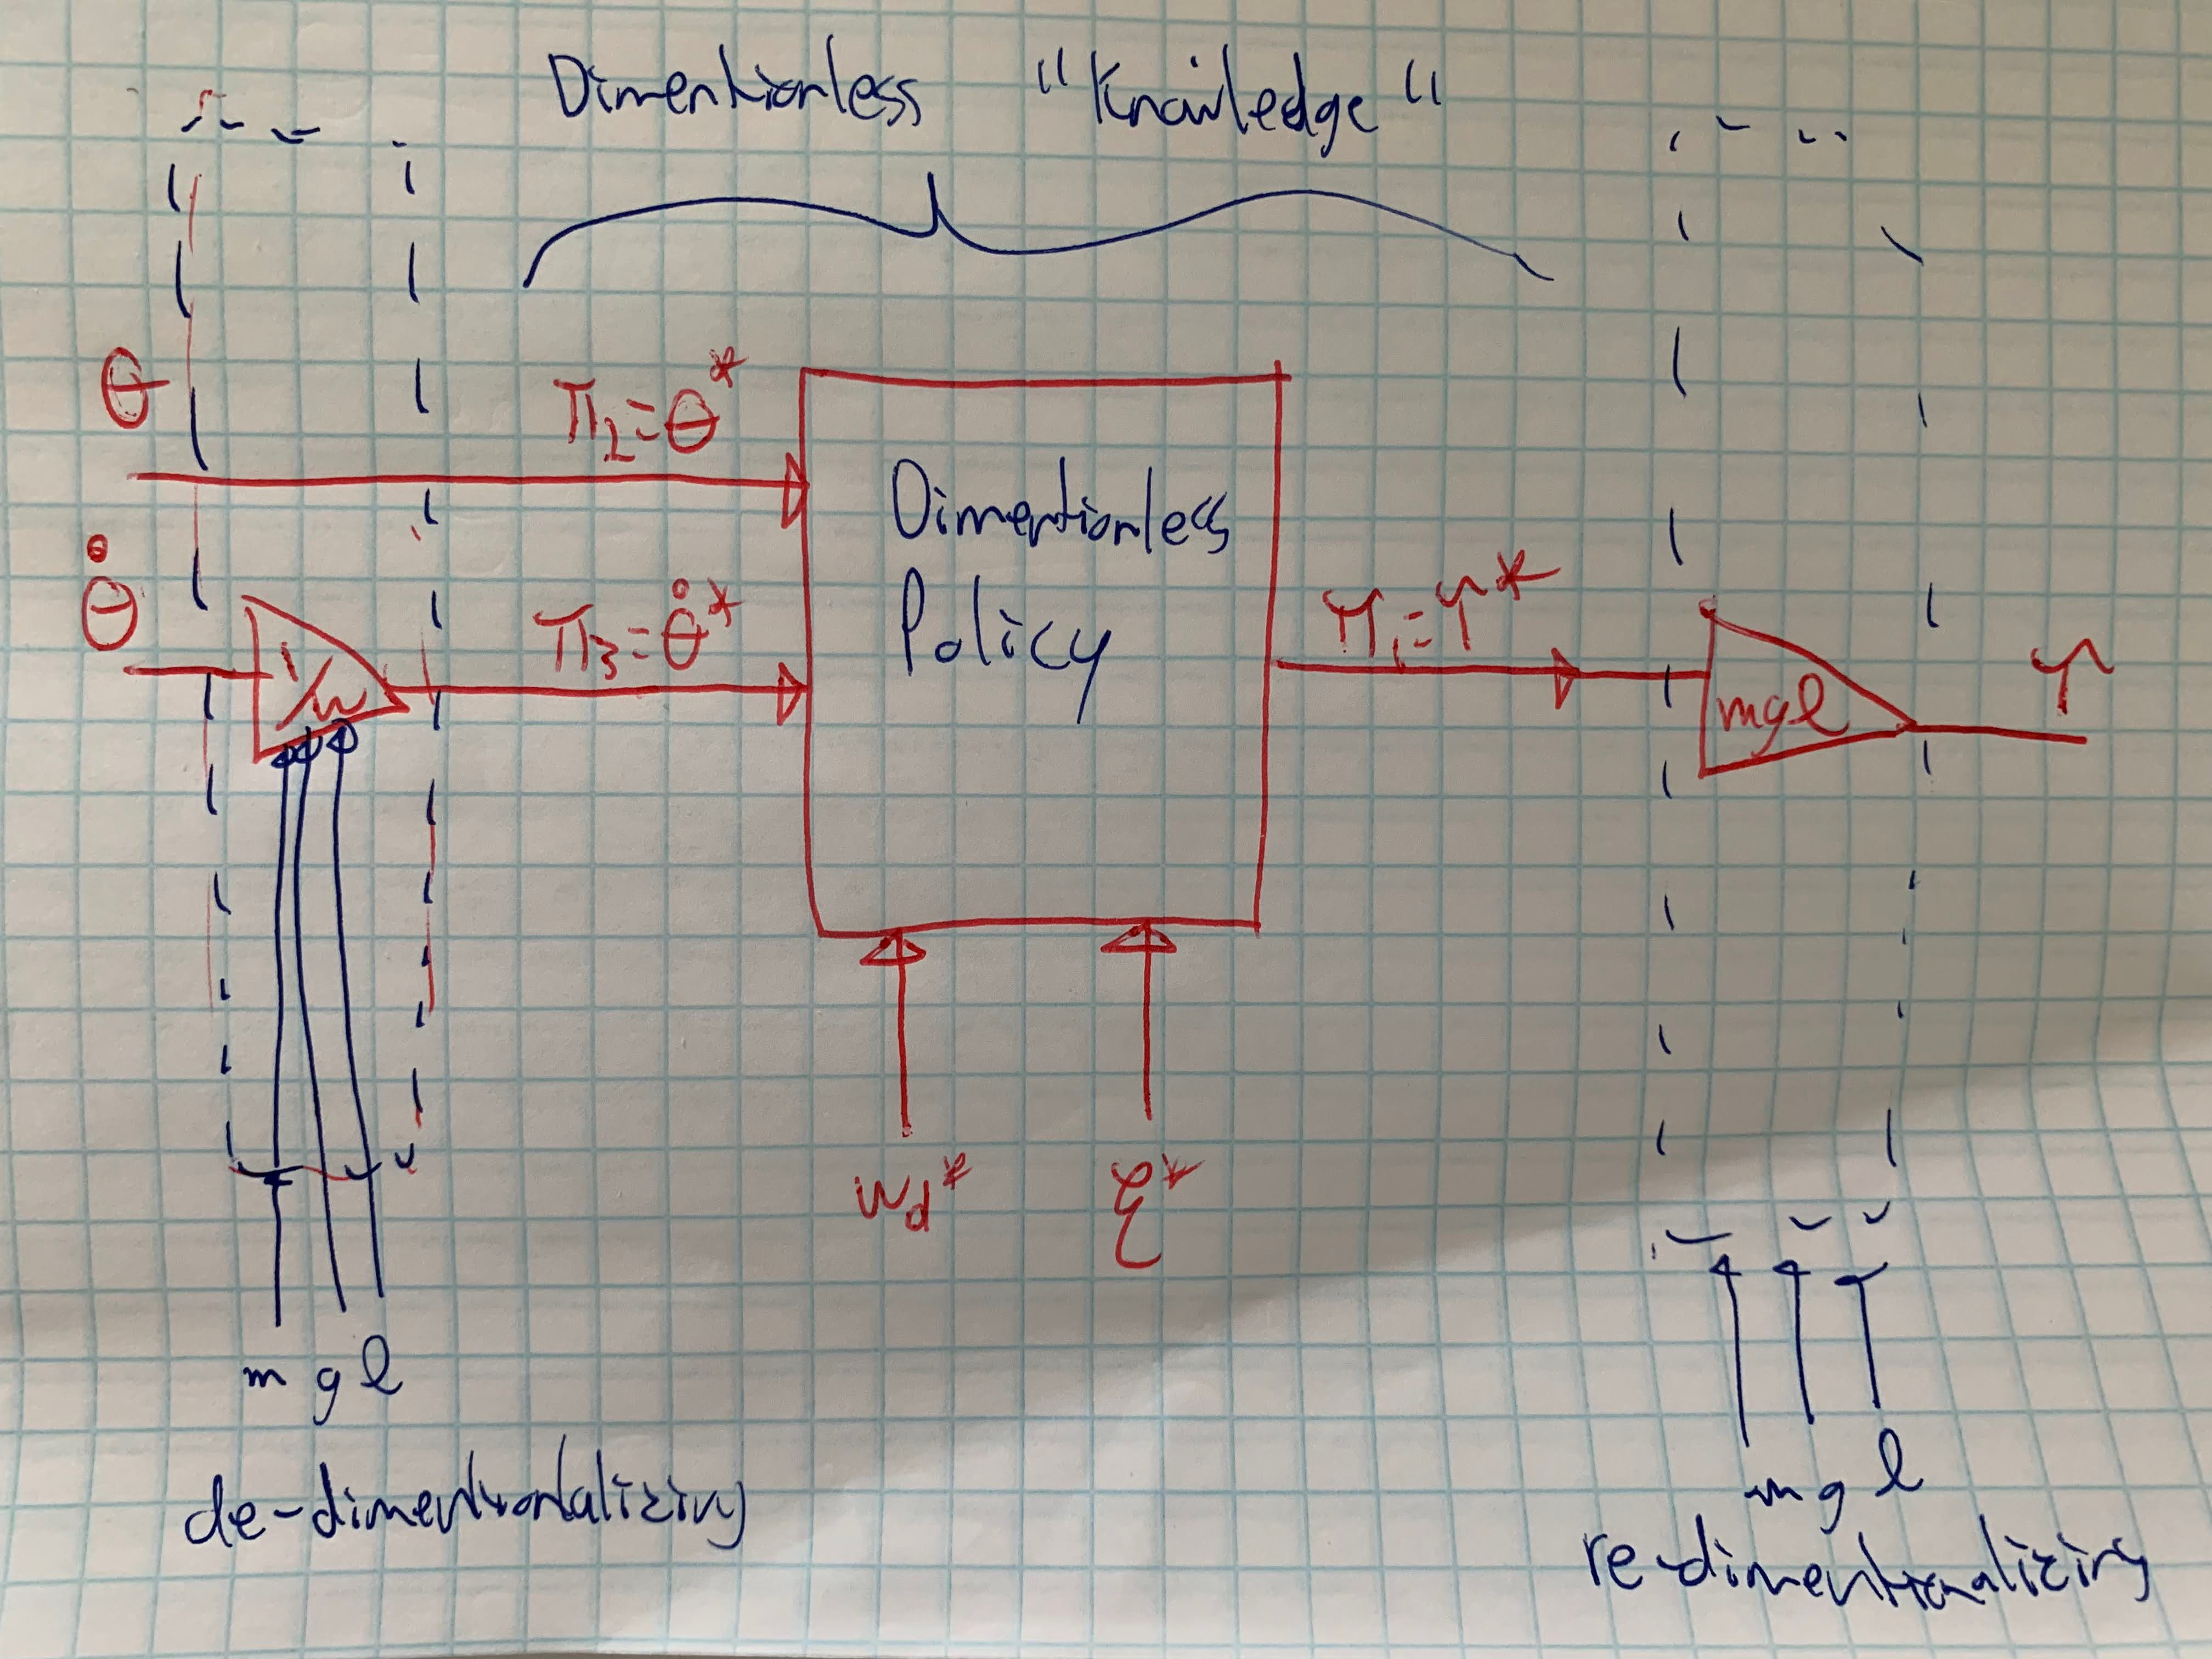
\includegraphics[width=0.99\linewidth]{fig/ct.JPG}
\caption{Dimentionless computed torque}\label{fig:ct}
\end{center}
\end{figure}
%%%%%%%%%%%%%%%%%%%%%%




\newpage
\subsection{Linear Quatratic Reglator (LQR) solution}


%%%%%%%%%%%%%%%%%%%%%%
\begin{equation}
\underbrace{\tau}_{\text{inputs}}
=
\pi \left(
\underbrace{ \theta, \dot{\theta} }_{\text{states}},
\underbrace{ m , g , l }_{\text{system parameters}},
\underbrace{ q }_{\text{policy parameters}}
\right)
\end{equation}
%%%%%%%%%%%%%%%%%%%%%%


\newpage
%%%%%%%%%%%%%%%%%%%%%%
\section{Numerical optimal policies}

%%%%%%%%%%%%%%%%%%%%%%%%%%%%%%%%%%%%%%%%%%%%
\begin{table}[htb]
   \centering % center the table
   \caption{Pendulum swing-up problems parameters} 
   \begin{tabular}{ p{2.0cm} p{0.8cm} p{0.8cm} p{0.8cm} p{0.8cm} p{0.8cm} }
   \hline \hline \noalign{\smallskip} \noalign{\smallskip} 
   %%%%%%%%%%%%%%%%%%%%%%
      & $m$ & $g$ & $l$ & $q$ & $\tau_{max}$ \\ \hline
   %%%%%%%%%%%%%%%%%%%%%
   %%%%%%%%%%%%%%%%%%%%%%
   \hline \hline \noalign{\smallskip} 
   \multicolumn{6}{c}{\textbf{Problems with $\tau_{max}^* = 0.5$ and $q^* = 0.1$} }\\ \noalign{\smallskip}  \hline\hline  \noalign{\smallskip} 
   %%%%%%%%%%%%%%%%%%%%%%
   Context no 1 : & 1.0 & 10.0 & 1.0 & 1.0 & 5.0 \\
   Context no 2 : & 1.0 & 10.0 & 2.0 & 2.0 & 10.0 \\
   Context no 3 : & 2.0 & 10.0 & 1.0 & 2.0 & 10.0 \\
   %%%%%%%%%%%%%%%%%%%%%
   \hline \hline \noalign{\smallskip} 
   \multicolumn{6}{c}{\textbf{Problems with $\tau_{max}^* = 1.0$ and $q^* = 0.05$} }\\ \noalign{\smallskip}  \hline\hline  \noalign{\smallskip} 
   %%%%%%%%%%%%%%%%%%%%%%
   Context no 4 : & 1.0 & 10.0 & 1.0 & 0.5 & 10.0 \\
   Context no 5 : & 1.0 & 10.0 & 2.0 & 1.0 & 20.0 \\
   Context no 6 : & 2.0 & 10.0 & 1.0 & 1.0 & 20.0 \\
   %%%%%%%%%%%%%%%%%%%%%
   \hline \hline \noalign{\smallskip} 
   \multicolumn{6}{c}{\textbf{Problems with $\tau_{max}^* = 1.0$ and $q^* = 10$} }\\ \noalign{\smallskip}  \hline\hline  \noalign{\smallskip} 
   %%%%%%%%%%%%%%%%%%%%%%
   Context no 7 : & 1.0 & 10.0 & 1.0 & 100.0 & 10.0 \\
   Context no 8 : & 1.0 & 10.0 & 2.0 & 200.0 & 20.0 \\
   Context no 9 : & 2.0 & 10.0 & 1.0 & 200.0 & 20.0 \\
   %%%%%%%%%%%%%%%%%%%%%
   \hline \hline
   \end{tabular}
\end{table}
%%%%%%%%%%%%%%%%%%%%%%%%%%%%%%%%%%%%%%%%%%%%

\subsection{Additionnal dimentionless parameters for the solver}

Using dynamic programming for solving the optimal policy numerically require setting additionnal parameter that define the domain. Altough those parameter should not affect the optimal policy far away from the boundaries, here a dimensionless version of those parameters was kept fixed in all the experiments:
%%%%%%%%%%%%%%%%%%%%%%
\begin{align}
\theta^*_{max} &= \theta_{max} = 2 \pi \\
\dot{\theta}^*_{max} &= \frac{ \dot{\theta}_{max} }{\omega} = 2 \\
t^*_{f} &= t_{f} \; \omega = 10 \times 2 \pi 
\end{align}
%%%%%%%%%%%%%%%%%%%%%%
$\theta_{max}$ is the range of angle for witch the optimal policy is solved, here set at one full revolution. $\dot{\theta}_{max}$ is the range of angular velocity for witch the optimal policy is solved, here the dimentionless ratio scaled with the natural frequency is set at 2. $t_{f}$ is the time horizon, here its associated dimentionless ratio is fixed to always corespond to 10 periods of the pendulum using the natural frequency.






\newpage

%%%%%%%%%%%%%%%%%%%%%%
\begin{equation}
\tau^*
=
\pi^* \left(
\theta, \dot{\theta}^*,
q^*=0.1 , \tau_{max}^* = 0.5
\right)
\end{equation}
%%%%%%%%%%%%%%%%%%%%%%

%%%%%%%%%%%%%%%%%%%%%%
\begin{figure}[H]
\begin{center}
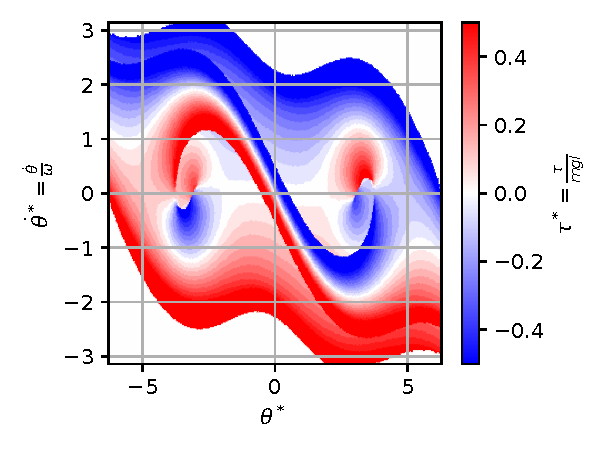
\includegraphics[width=0.99\linewidth]{fig/c1_dimpolicy.pdf}
\caption{Context no 1, 2 and 4 dimentionless optimal policy}\label{fig:c1_policy}
\end{center}
\end{figure}
%%%%%%%%%%%%%%%%%%%%%%

%%%%%%%%%%%%%%%%%%%%%%
\begin{equation}
\tau^*
=
\pi^* \left(
\theta, \dot{\theta}^*,
q^*=0.05 , \tau_{max}^* = 1.0
\right)
\end{equation}
%%%%%%%%%%%%%%%%%%%%%%

%%%%%%%%%%%%%%%%%%%%%%
\begin{figure}[H]
\begin{center}
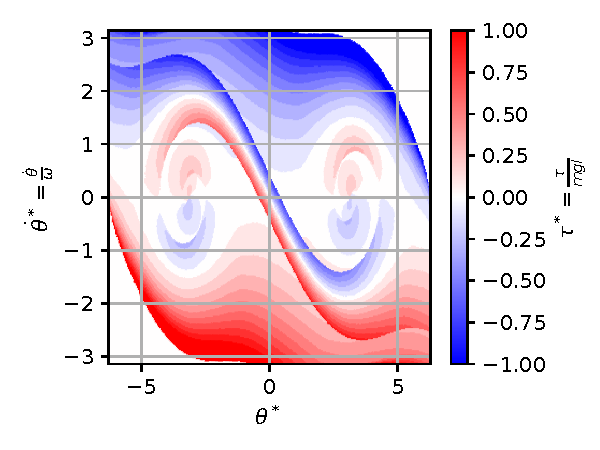
\includegraphics[width=0.99\linewidth]{fig/c4_dimpolicy.pdf}
\caption{Context no 4, 5 and 6 dimentionless optimal policy}\label{fig:c1_policy}
\end{center}
\end{figure}
%%%%%%%%%%%%%%%%%%%%%%

%%%%%%%%%%%%%%%%%%%%%%
\begin{equation}
\tau^*
=
\pi^* \left(
\theta, \dot{\theta}^*,
q^* = 10 , \tau_{max}^* = 1.0
\right)
\end{equation}
%%%%%%%%%%%%%%%%%%%%%%
%%%%%%%%%%%%%%%%%%%%%%
\begin{figure}[H]
\begin{center}
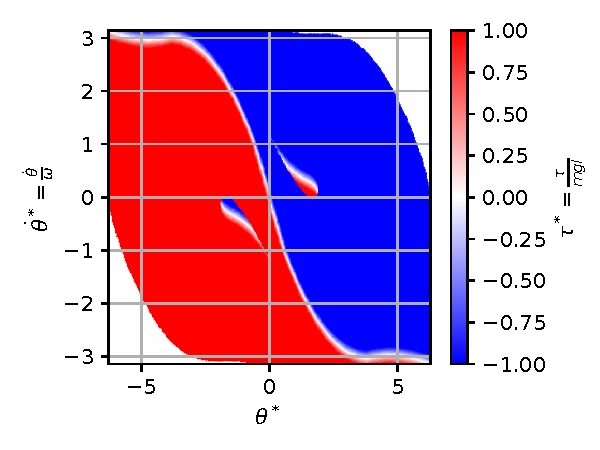
\includegraphics[width=0.99\linewidth]{fig/c7_dimpolicy.pdf}
\caption{Context no 7, 8 and 9 dimentionless optimal policy}\label{fig:c1_policy}
\end{center}
\end{figure}
%%%%%%%%%%%%%%%%%%%%%%












%  \begin{figure}[ht]
%     \centering
%     \vspace{-10pt}
%     \subfloat[Small vehicle \label{fig:a}]{\includegraphics[width=0.12\textwidth]{fig/a.jpg}}
%     \subfloat[Long vehicle \label{fig:b}]{\includegraphics[width=0.18\textwidth]{fig/b.jpg}}   
%     \subfloat[Large vehicle \label{fig:c}]{\includegraphics[width=0.16\textwidth]{fig/c.PNG}}
%     \caption{subfigures}
%     \label{fig:subfigures}
% \end{figure}











%%%%%%%%%%%%%%%%%%%%%%
\begin{figure}[p]
\begin{center}
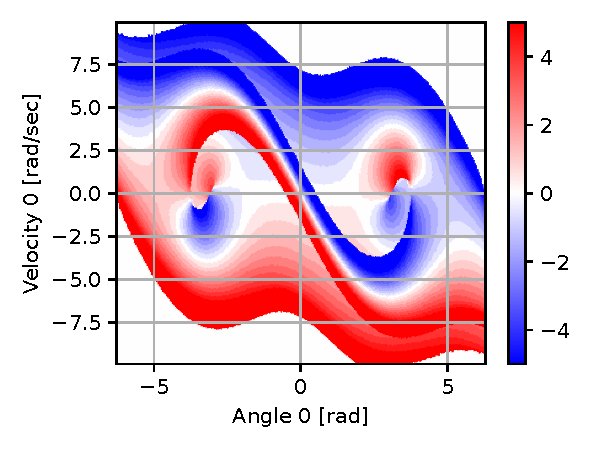
\includegraphics[width=0.99\linewidth]{fig/c1_policy.pdf}
\caption{Context no 1 optimal policy}\label{fig:c1_policy}
\end{center}
\end{figure}
%%%%%%%%%%%%%%%%%%%%%%


%%%%%%%%%%%%%%%%%%%%%%
\begin{figure}[p]
\begin{center}
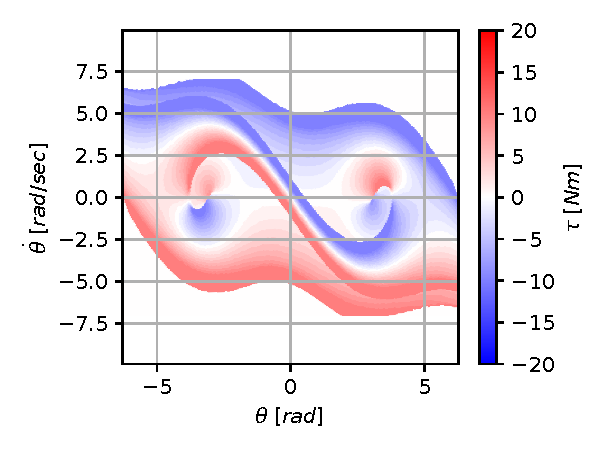
\includegraphics[width=0.99\linewidth]{fig/c2_policy.pdf}
\caption{Context no2 optimal policy}\label{fig:c1_policy}
\end{center}
\end{figure}
%%%%%%%%%%%%%%%%%%%%%%

%%%%%%%%%%%%%%%%%%%%%%
\begin{figure}[p]
\begin{center}
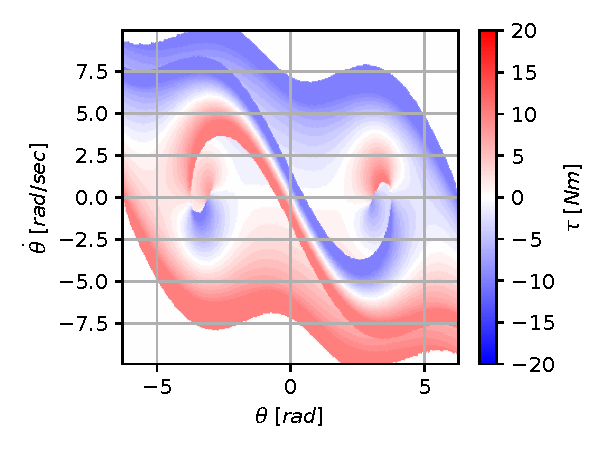
\includegraphics[width=0.99\linewidth]{fig/c3_policy.pdf}
\caption{Context no3 optimal policy}\label{fig:c1_policy}
\end{center}
\end{figure}
%%%%%%%%%%%%%%%%%%%%%%

\newpage
%%%%%%%%%%%%%%%%%%%%%%
\begin{figure}[p]
\begin{center}
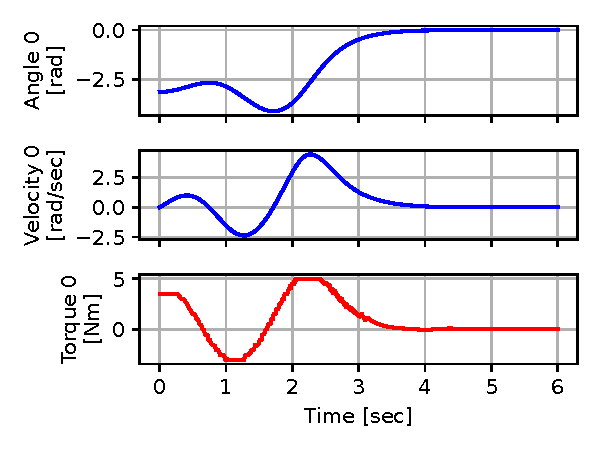
\includegraphics[width=0.99\linewidth]{fig/c1_traj.pdf}
\caption{Context no1 optimal trajectory from up-down position}\label{fig:c1_traj}
\end{center}
\end{figure}
%%%%%%%%%%%%%%%%%%%%%%


%%%%%%%%%%%%%%%%%%%%%%
\begin{figure}[p]
\begin{center}
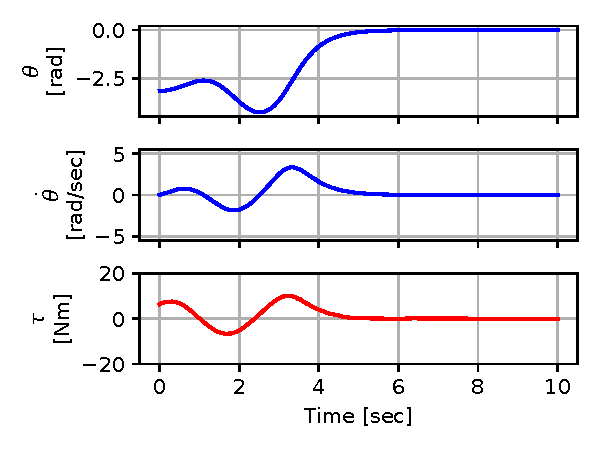
\includegraphics[width=0.99\linewidth]{fig/c2_traj.pdf}
\caption{Context no2 optimal trajectory from up-down position}\label{fig:c2_traj}
\end{center}
\end{figure}
%%%%%%%%%%%%%%%%%%%%%%

%%%%%%%%%%%%%%%%%%%%%%
\begin{figure}[p]
\begin{center}
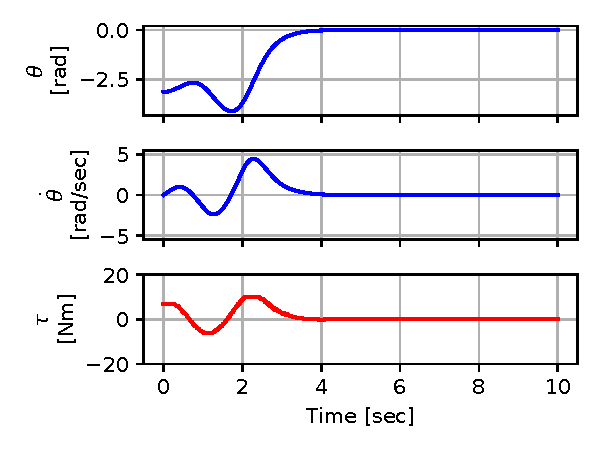
\includegraphics[width=0.99\linewidth]{fig/c3_traj.pdf}
\caption{Context no3 optimal trajectory from up-down position}\label{fig:c3_traj}
\end{center}
\end{figure}
%%%%%%%%%%%%%%%%%%%%%%


%%%%%%%%%%%%%%%%%%%%%%
\begin{figure}[p]
\begin{center}
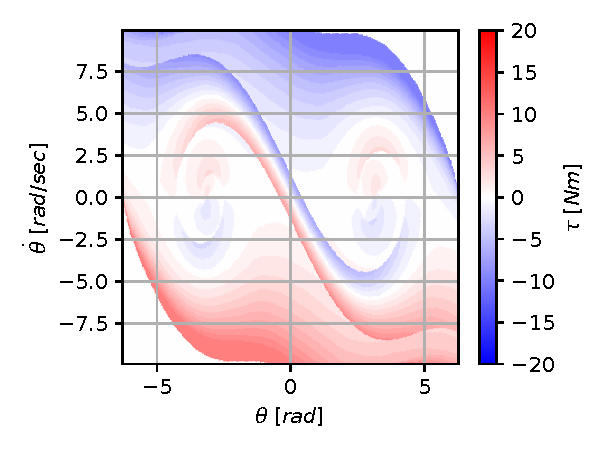
\includegraphics[width=0.99\linewidth]{fig/c4_policy.pdf}
\caption{Context no 4 optimal policy}\label{fig:c4_policy}
\end{center}
\end{figure}
%%%%%%%%%%%%%%%%%%%%%%


%%%%%%%%%%%%%%%%%%%%%%
\begin{figure}[p]
\begin{center}
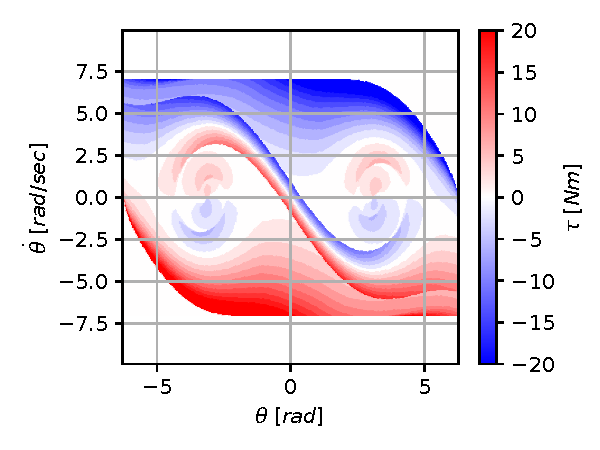
\includegraphics[width=0.99\linewidth]{fig/c5_policy.pdf}
\caption{Context no5 optimal policy}\label{fig:c5_policy}
\end{center}
\end{figure}
%%%%%%%%%%%%%%%%%%%%%%

%%%%%%%%%%%%%%%%%%%%%%
\begin{figure}[p]
\begin{center}
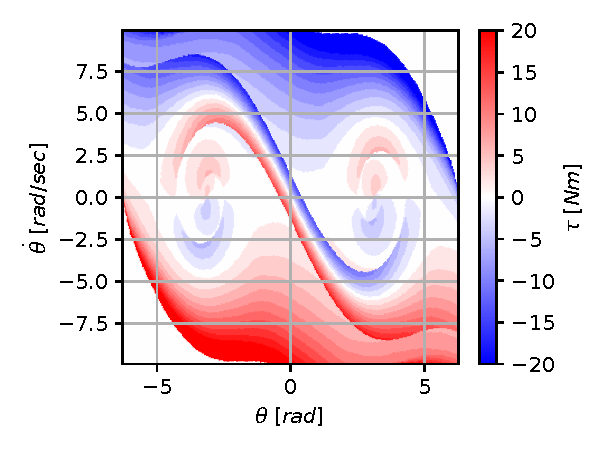
\includegraphics[width=0.99\linewidth]{fig/c6_policy.pdf}
\caption{Context no6 optimal policy}\label{fig:c6_policy}
\end{center}
\end{figure}
%%%%%%%%%%%%%%%%%%%%%%

\newpage
%%%%%%%%%%%%%%%%%%%%%%
\begin{figure}[p]
\begin{center}
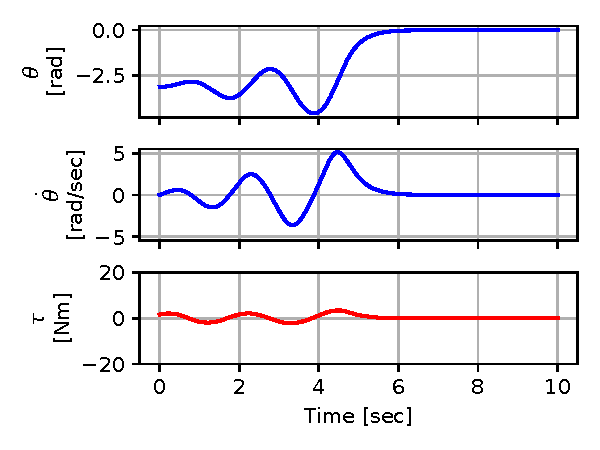
\includegraphics[width=0.99\linewidth]{fig/c4_traj.pdf}
\caption{Context no4 optimal trajectory from up-down position}\label{fig:c4_traj}
\end{center}
\end{figure}
%%%%%%%%%%%%%%%%%%%%%%


%%%%%%%%%%%%%%%%%%%%%%
\begin{figure}[p]
\begin{center}
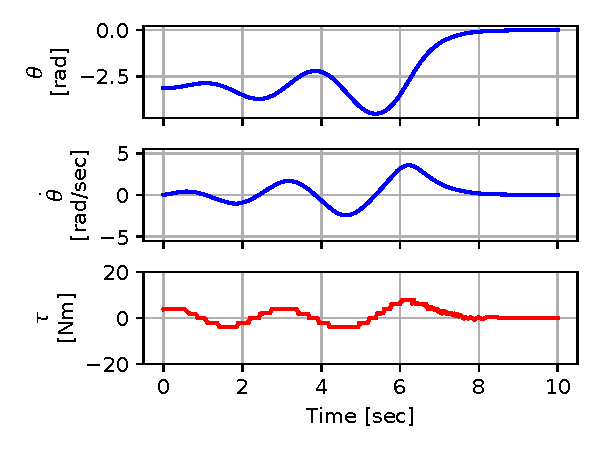
\includegraphics[width=0.99\linewidth]{fig/c5_traj.pdf}
\caption{Context no5 optimal trajectory from up-down position}\label{fig:c5_traj}
\end{center}
\end{figure}
%%%%%%%%%%%%%%%%%%%%%%

%%%%%%%%%%%%%%%%%%%%%%
\begin{figure}[p]
\begin{center}
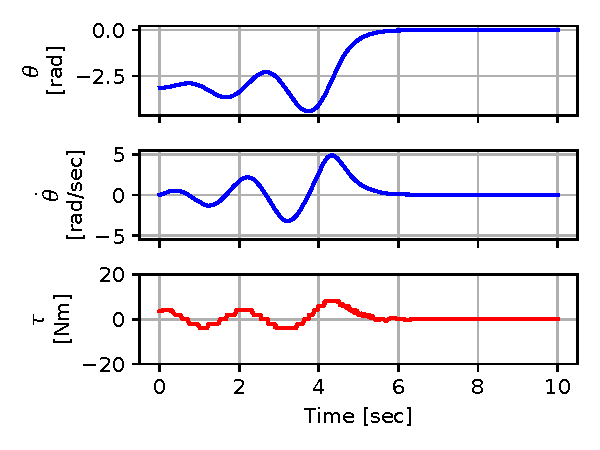
\includegraphics[width=0.99\linewidth]{fig/c6_traj.pdf}
\caption{Context no6 optimal trajectory from up-down position}\label{fig:c6_traj}
\end{center}
\end{figure}
%%%%%%%%%%%%%%%%%%%%%%


%%%%%%%%%%%%%%%%%%%%%%
\begin{figure}[p]
\begin{center}
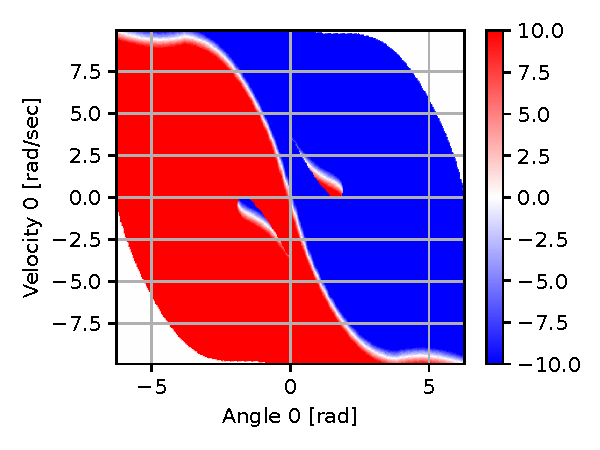
\includegraphics[width=0.99\linewidth]{fig/c7_policy.pdf}
\caption{Context no 7 optimal policy}\label{fig:c7_policy}
\end{center}
\end{figure}
%%%%%%%%%%%%%%%%%%%%%%


%%%%%%%%%%%%%%%%%%%%%%
\begin{figure}[p]
\begin{center}
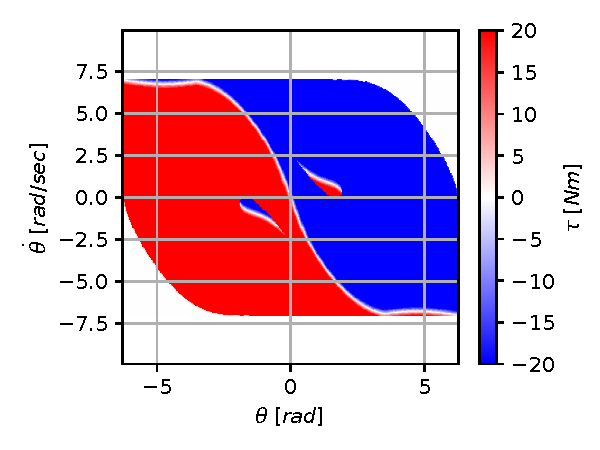
\includegraphics[width=0.99\linewidth]{fig/c8_policy.pdf}
\caption{Context no8 optimal policy}\label{fig:c8_policy}
\end{center}
\end{figure}
%%%%%%%%%%%%%%%%%%%%%%

%%%%%%%%%%%%%%%%%%%%%%
\begin{figure}[p]
\begin{center}
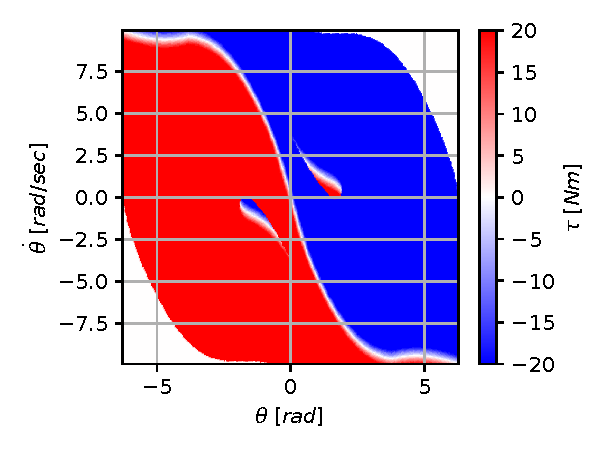
\includegraphics[width=0.99\linewidth]{fig/c9_policy.pdf}
\caption{Context no9 optimal policy}\label{fig:c9_policy}
\end{center}
\end{figure}
%%%%%%%%%%%%%%%%%%%%%%

\newpage
%%%%%%%%%%%%%%%%%%%%%%
\begin{figure}[p]
\begin{center}
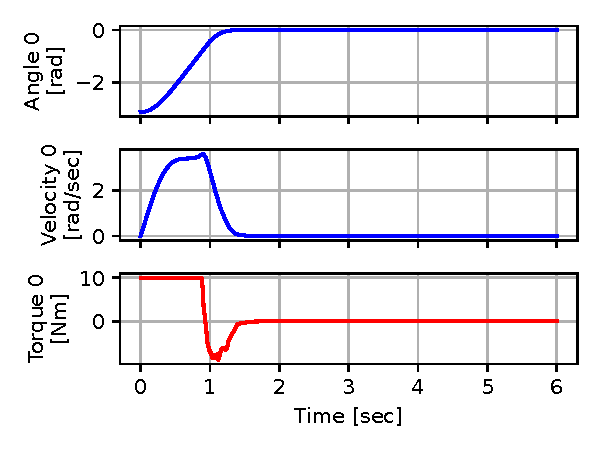
\includegraphics[width=0.99\linewidth]{fig/c7_traj.pdf}
\caption{Context no7 optimal trajectory from up-down position}\label{fig:c7_traj}
\end{center}
\end{figure}
%%%%%%%%%%%%%%%%%%%%%%


%%%%%%%%%%%%%%%%%%%%%%
\begin{figure}[p]
\begin{center}
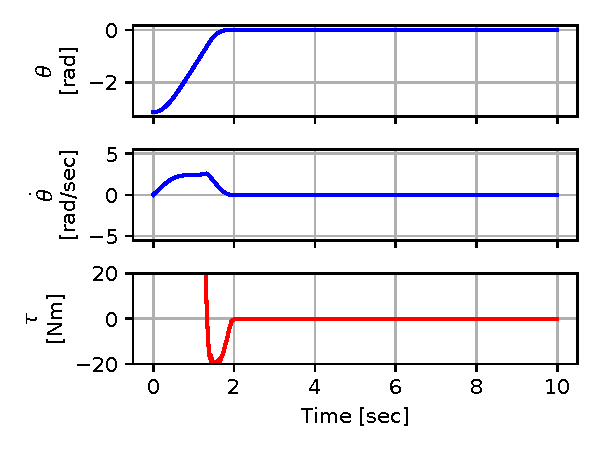
\includegraphics[width=0.99\linewidth]{fig/c8_traj.pdf}
\caption{Context no8 optimal trajectory from up-down position}\label{fig:c8_traj}
\end{center}
\end{figure}
%%%%%%%%%%%%%%%%%%%%%%

%%%%%%%%%%%%%%%%%%%%%%
\begin{figure}[p]
\begin{center}
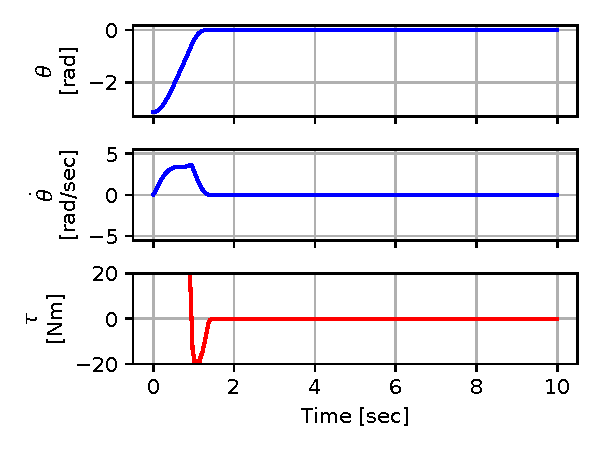
\includegraphics[width=0.99\linewidth]{fig/c9_traj.pdf}
\caption{Context no9 optimal trajectory from up-down position}\label{fig:c9_traj}
\end{center}
\end{figure}
%%%%%%%%%%%%%%%%%%%%%%



